% Drawing 148/01-14 -- folder 148, batch 01, archive page 17 (PDF page 18).
% Transcription: en bas à gauche, une sphère au crayon : l'équateur à l'encre, tracé en entier, portant quatre points ; deux méridiens en rouge passant chacun par deux de ces points.
% Kind: sphere with equator, four points and two red meridians. Method 2 (schematic redraw from the facsimile). Status: ok.
% Notes: Colour render. Faint pencil outline; the equator a full heavy ink ellipse with four dots on it (two on the back half, two on the front half), each placed on the ellipse; two red meridians from the top to the bottom of the outline, the left one through the two left dots (dashed above the equator, where it runs on the back), the right one through the two right dots (doubled in black ink on the page, drawn once). Redrawn 2026-11-12 (issue 128): to check again.
% Coordinates: 1 unit = 1 mm = 1/100 of the crop width, y downwards as on the crop (bbox in page fractions: [0.21, 0.76, 0.4, 0.875]).
% Redrawn by Claude (claude-fable-5-2), issue #128, 2026-11-12; not checked by a human; not compiled (no TeX in the session).
% Rights: reproduces part of the work -- behind RENDER_TRANSCRIPTS, never published by itself.
\documentclass[tikz,border=3pt]{standalone}
\usepackage{amsmath,amssymb}
\usetikzlibrary{patterns,arrows.meta}
\tikzset{pencil/.style={black!45}, struck/.style={black!35}, mpt/.style={circle,draw,inner sep=1.3pt}, pt/.style={circle,fill,inner sep=0.9pt}, opt/.style={circle,draw,fill=white,inner sep=1.1pt}, Rd/.style={red!75!black}, Gn/.style={green!45!black}, Br/.style={brown!70!black}}
\begin{document}
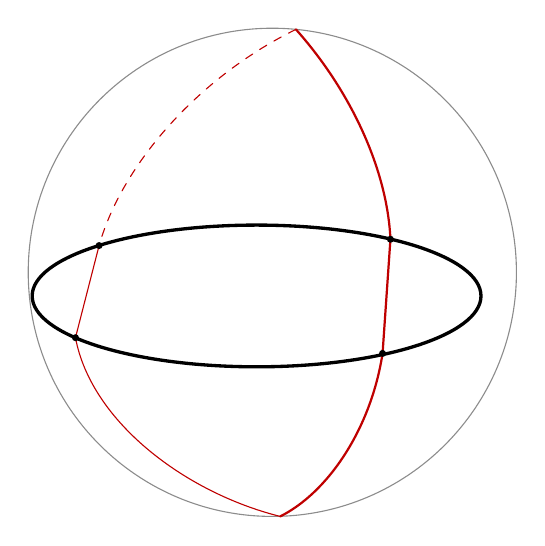
\begin{tikzpicture}[x=1mm,y=-1mm,line cap=round,line join=round,font=\small]
\draw[pencil] (51,42) circle [radius=31];
\draw[very thick] (49,45) ellipse [x radius=28.5, y radius=9];
\coordinate (N) at (54,11.15);
\coordinate (S) at (52,73);
\coordinate (a) at (29,38.6);
\coordinate (b) at (66,37.8);
\coordinate (c) at (26,50.3);
\coordinate (d) at (65,52.3);
\draw[Rd,dashed] (N) .. controls (42,17) and (32,28) .. (a);
\draw[Rd] (a) -- (c) .. controls (28,61) and (40,70) .. (S);
\draw[Rd,thick] (N) .. controls (61,19) and (65.6,29) .. (b) -- (d) .. controls (63.5,62) and (58,70) .. (S);
\node[pt] at (a) {};
\node[pt] at (b) {};
\node[pt] at (c) {};
\node[pt] at (d) {};
\end{tikzpicture}
\end{document}
